\chapter{参数化、有效几何与跨宽度迁移}
\label{l5:chapter}

前四讲研究了一个给定目标函数上的更新规则：如何利用凸性、对偶结构、随机梯度、动量和矩阵几何选择下一步。本讲把问题再向前推进一步。神经网络的目标函数并不是独立于模型设计的对象；我们选择宽度、层数、输出缩放和参数坐标时，也在选择优化器实际面对的几何。同一个输入输出映射可以有不同的参数表示，而同一个名为 SGD 的算法，在这些表示上通常会产生不同的函数轨迹。

本讲围绕一个可计算的问题展开：\emph{一次参数更新，在训练样本的预测上产生了什么更新？}答案由模型的 Jacobian、优化器的几何和数据共同决定。我们先得到 $JPJ^\top$，再用两个可以手算的模型理解它，最后用一套记号推导两层网络的宽度尺度。这样，NTK、特征学习、$\mu$P 和隐式偏好就能与前面学习的条件数、预条件和稳定性连接起来。

\begin{coursebox}{学习目标与本讲边界}
学完本讲，应当能够完成以下任务。
\begin{enumerate}
  \item 从参数更新推导训练预测的局部更新，区分精确梯度流恒等式与有限步长近似。
  \item 用有效核的特征值及目标在其特征向量上的投影，解释哪些数据方向学得快。
  \item 推导两层矩阵分解诱导的预条件，写出正确的内部 Gram 平衡条件。
  \item 在明确的两层模型中，推导 NTP 与 mean-field 参数化的 SGD 学习率尺度，并换算实际输出权重的学习率。
  \item 设计跨宽度学习率扫描，利用特征变化和验证误差诊断迁移，区分隐式偏好与泛化保证。
\end{enumerate}
本讲的尺度定理以无动量 SGD 为主。Adam 的状态、$\epsilon$、参数组和权重衰减需要另行约定；Muon 的矩阵更新也不能直接塞进一个固定的正定预条件矩阵。完整的深层 $\mu$P 规则、均值场偏微分方程与全局损失拓扑属于选读。
\end{coursebox}

\section{教学路线与实验安排}
\label{l5:route}

本讲安排为 \textbf{1.5 学时理论与 1.5 学时实验}。以下学时均指课程计划中的学时单位。讲义保留了完整推导和习题解答，课堂不需要逐行讲完所有选读证明。

\begin{center}
\begin{tabularx}{\textwidth}{@{}p{0.13\textwidth}X p{0.15\textwidth}@{}}
\toprule
环节 & 核心任务 & 建议学时 \\
\midrule
理论一 & 预测空间更新、有效核与目标方向 & $0.30$ \\
理论二 & 矩阵分解诱导几何与平衡条件 & $0.30$ \\
理论三 & 固定核模型、两层宽度尺度、输出坐标换算 & $0.60$ \\
理论四 & 迁移诊断、隐式偏好与稳定性边界 & $0.30$ \\
\midrule
实验一 & 固定数据、中心化输出、检查损失及参数组 & $0.25$ \\
实验二 & 固定步数与 batch，进行宽度和基础学习率扫描 & $0.50$ \\
实验三 & 解释特征 Gram 漂移与每参数变化，复核迁移 & $0.50$ \\
实验四 & 写出有条件的结论与失败原因 & $0.25$ \\
\bottomrule
\end{tabularx}
\end{center}

理论课必须讲清的三个等式是预测更新中的 $JPJ^\top$、矩阵分解中的内部 Gram 平衡，以及 $b=a/m$ 引起的学习率坐标变换。固定核误差公式可以作为前面谱分解知识的应用。关于有限步长平衡误差、Adam 坐标换算和局部 Hessian 的细节，可根据学生基础安排为课后阅读。

\section{从参数更新到预测更新}
\label{l5:effective-geometry}

\subsection{数据、参数与损失的统一记号}

固定训练集 $\{(x_i,y_i)\}_{i=1}^n$。先考虑标量输出网络 $f_\theta(x)$，参数向量 $\theta\in\R^p$。定义训练预测向量、残差与平均平方损失：
\begin{equation}
 F(\theta)=\begin{pmatrix}f_\theta(x_1)\\ \vdots\\ f_\theta(x_n)\end{pmatrix},
 \qquad r(\theta)=F(\theta)-y,
 \qquad L(\theta)=\frac{1}{2n}\norm{r(\theta)}_2^2.
 \label{l5:loss}
\end{equation}
记训练预测的 Jacobian 为
\begin{equation}
 J(\theta)=\frac{\partial F(\theta)}{\partial\theta}
 \in\R^{n\times p},
 \qquad \nabla_\theta L(\theta)=\frac1nJ(\theta)^\top r(\theta).
 \label{l5:jacobian}
\end{equation}
矩阵 $J$ 的第 $i$ 行描述：参数如何改变第 $i$ 个训练样本的预测。$J$ 同时依赖模型结构、当前参数和输入数据，因此仅从参数个数不能判断训练的难易。

本讲使用可微激活函数来书写导数，实验采用 $\tanh$。对 ReLU，可在可微区域作相同的局部计算，但不能在折点上直接套用需要二阶连续可微的结论。

\subsection{预条件梯度流的精确恒等式}

设 $P(\theta)\in\R^{p\times p}$ 对称半正定，考虑连续时间系统
\begin{equation}
 \dot\theta=-P(\theta)\nabla_\theta L(\theta).
 \label{l5:parameter-flow}
\end{equation}
这里的 $P$ 可以是固定度量，也可以沿轨迹变化。只要解足够光滑，链式法则给出以下结果。

\begin{proposition}[预测空间中的有效核]
对式 \eqref{l5:parameter-flow}，有
\begin{equation}
 \dot r=-\frac1n\mathcal K(\theta)r,
 \qquad
 \boxed{\mathcal K(\theta)=J(\theta)P(\theta)J(\theta)^\top}.
 \label{l5:effective-kernel}
\end{equation}
有效核 $\mathcal K$ 对称半正定，且
\begin{equation}
 \frac{d}{dt}L(\theta(t))
 =-\frac1{n^2}r^\top\mathcal K r\leq0.
 \label{l5:loss-flow}
\end{equation}
\end{proposition}

\begin{proof}
由 $y$ 固定，$\dot r=J\dot\theta$。代入参数更新即得
$\dot r=-JPJ^\top r/n$。对任意 $v\in\R^n$，
$v^\top JPJ^\top v=(J^\top v)^\top P(J^\top v)\geq0$。
最后对 $\norm r^2/(2n)$ 求导即可。这个证明没有用到 $P$ 的导数，因为此处计算的是轨迹的一阶变化。
\end{proof}

这一恒等式把三类设计选择写在了同一个地方：数据决定 $J$ 在哪些输入上求值，架构和参数化决定 $J$ 的列，优化器的瞬时度量决定 $P$。它说明了为何优化器与网络不能总是分开讨论。但它没有保证 $\mathcal K$ 始终良态：核可能退化，某些目标方向可能几乎位于其零空间，核自身也可能迅速改变。

\begin{remark}[哪些算法可以直接使用这个公式]
普通梯度流对应 $P=I$，固定对角或矩阵预条件梯度流也符合上述形式。带动量的算法有额外状态，更新方向通常不是当前梯度乘一个预先给定的对称半正定矩阵。Adam 同时具有一阶矩、二阶矩和 $\epsilon$；Muon 则对动量矩阵作非线性谱变换。分析它们时，可以研究局部线性化或完整状态更新，但不能默认所有动力学都精确地由同一个 $JPJ^\top$ 描述。
\end{remark}

\subsection{有限步长：有效核只描述一阶项}

实际梯度更新为
\begin{equation}
 \theta^+=\theta+\Delta\theta,
 \qquad \Delta\theta=-\frac\eta nP J^\top r.
\end{equation}
Taylor 展开得到
\begin{equation}
 r^+=\left(I-\frac\eta n\mathcal K(\theta)\right)r+R,
 \label{l5:discrete-kernel}
\end{equation}
其中 $R$ 是预测映射的非线性余项。例如，若更新线段上每个 $f_\theta(x_i)$ 的参数 Hessian 算子范数不超过 $B_i$，则
\begin{equation}
 |R_i|\leq\frac{B_i}{2}\norm{\Delta\theta}_2^2,
 \qquad
 \norm R_2\leq\frac12\left(\sum_iB_i^2\right)^{1/2}
 \norm{\Delta\theta}_2^2.
\end{equation}
因此，步长小、预测对参数接近线性，或者能另行控制余项时，式 \eqref{l5:discrete-kernel} 的核项才是可靠的单步近似。大步长下必须检查余项，不能把梯度流的单调下降直接当成离散训练的性质。

对于 SGD，随机 batch 梯度在恰当抽样下可以是全梯度的无偏估计，但经过非线性参数更新之后，下一步预测的期望并不等于把期望梯度代入整个非线性网络。第3讲关于条件期望和噪声的区分在这里仍然适用。

\subsection{重参数化本身就是一种预条件}

设用新参数 $u$ 表示原参数 $\theta=\phi(u)$，对 $u$ 做欧氏梯度流。记 $D\phi$ 为坐标映射的 Jacobian，则
\begin{equation}
 \dot u=-D\phi(u)^\top\nabla_\theta L,
 \qquad
 \dot\theta=-D\phi(u)D\phi(u)^\top\nabla_\theta L.
 \label{l5:reparameterization}
\end{equation}
因此原坐标中出现了 $P=D\phi D\phi^\top$。若 $\phi$ 是线性可逆变换，这就是一个固定正定预条件；若 $\phi$ 非线性或引入冗余参数，$P$ 可以随训练改变并且可能退化。

\begin{coursebox}{课程主线}
“同样使用 SGD”并不表示“同样的优化方法”。要比较两个训练配置，至少需要写出前向参数化、实际存储的变量、各参数组学习率和损失归一化。只有这些约定明确，学习率数值与条件数的比较才有意义。
\end{coursebox}

\section{架构应当适配哪些数据方向}
\label{l5:target-directions}

\subsection{核谱与残差投影必须一起看}

暂时假设 $\mathcal K$ 不随时间改变，记归一化有效核为
$\Theta=\mathcal K/n$。设其特征分解为
\begin{equation}
 \Theta=Q\diag(\lambda_1,\ldots,\lambda_n)Q^\top,
 \qquad \lambda_j\geq0,
 \qquad c_j=q_j^\top r_0.
\end{equation}
则梯度流与离散线性模型分别满足
\begin{align}
 r(t)&=\sum_j c_j e^{-\lambda_jt}q_j,\label{l5:continuous-modes}\\
 r_t&=\sum_j c_j(1-\eta\lambda_j)^tq_j.\label{l5:discrete-modes}
\end{align}
连续时间下，非零特征值越大，对应残差消失得越快；零特征值方向不会被这个固定核学到。离散时间必须比较 $|1-\eta\lambda_j|$：当所有 $\eta\lambda_j\leq1$ 时，更大的特征值对应更快的衰减；接近稳定区间另一端 $\eta\lambda_j=2$ 时，衰减反而变慢并伴随符号交替。最坏方向的速度与谱的两端有关，而一个特定任务是否真的困难，还取决于 $c_j$。

\begin{example}[同样的谱，完全不同的目标适配]
考虑两个归一化有效核
\[
 \Theta_A=\begin{pmatrix}9&0\\0&1\end{pmatrix},
 \qquad
 \Theta_B=\begin{pmatrix}1&0\\0&9\end{pmatrix}.
\]
它们的迹均为 $10$，条件数均为 $9$。设初始预测为零，目标 $y=(0,1)^\top$，所以 $r_0=(0,-1)^\top$。取 $\eta=0.1$，两者都满足 $0<\eta<2/9$。一步后
\[
 r_1^{A}=(0,-0.9)^\top,
 \qquad r_1^{B}=(0,-0.1)^\top.
\]
目标是两个样本上的预测值，故损失为 $\norm r^2/4$。两种模型更新一次后的损失分别是 $0.2025$ 和 $0.0025$，相差 $81$ 倍。连续时间下，相应残差范数分别为 $e^{-t}$ 和 $e^{-9t}$。

如果目标改为 $y=(1,0)^\top$，结论恰好交换。这说明核的迹、平均特征值，甚至完整的特征值集合，都不足以单独判断对一个监督任务的适配程度。还需要知道目标在特征向量上的投影。
\end{example}

这个例子提供了一个具体的架构设计问题：结构先验是否把任务中有用的变化方向放到了容易学习的子空间？平移等变结构、局部连接或因子分解可以改变这种方向性，但是否有益需要结合数据和目标检验。不能只因参数更多、核更大，便宣布架构更适配数据。

\subsection{固定预条件也会改变最终选解}

回到线性预测 $F(w)=Xw$。假设 $X\in\R^{n\times d}$ 满行秩、$n<d$，固定 $P\succ0$，并从 $w_0=0$ 出发作预条件 GD：
\[
 w_{t+1}=w_t-\frac\eta nP X^\top(Xw_t-y).
\]
若 $0<\eta<2n/\lambda_{\max}(XPX^\top)$，则
\begin{equation}
 w_\infty=P X^\top(XPX^\top)^{-1}y
 =\argmin_{Xw=y}\frac12w^\top P^{-1}w.
 \label{l5:weighted-min-norm}
\end{equation}
这是第1讲最小范数结论在不同度量中的版本。证明只需令 $w=P^{1/2}u$，对设计矩阵 $XP^{1/2}$ 使用欧氏最小范数结论。这里改变的不仅是速度，还包括欠定问题中被选中的解。

\begin{example}[选解偏好与数据是否匹配]
令
\[
 X=\begin{pmatrix}1&0&1\\0&2&0\end{pmatrix},
 \qquad y=\begin{pmatrix}1\\2\end{pmatrix}.
\]
所有插值解都满足 $w_1+w_3=1,w_2=1$。普通 GD 从零出发，选择
$w^{I}=(1/2,1,1/2)^\top$。若 $P=\diag(4,1,1)$，则
\[
 XPX^\top=\begin{pmatrix}5&0\\0&4\end{pmatrix},
 \qquad
 w^{P}=\begin{pmatrix}4/5\\1\\1/5\end{pmatrix}.
\]
两者训练误差都为零。考虑新输入 $x_{\mathrm{new}}=(1,0,0)^\top$。如果真实参数是 $(1,1,0)^\top$，两个预测的绝对误差分别为 $1/2$ 和 $1/5$，预条件偏好更合适。如果真实参数是 $(0,1,1)^\top$，这两个真实参数仍生成相同的训练标签，但新输入上的误差变成 $1/2$ 和 $4/5$。

同一个优化器偏好，面对两个与训练集完全一致的真实规律，可以有不同的泛化结果。要判断哪个偏好更好，必须引入关于数据分布或目标结构的信息。
\end{example}

\section{深度矩阵分解如何诱导预条件}
\label{l5:factorization}

\subsection{同一个端到端矩阵，两种优化坐标}

令端到端矩阵 $W\in\R^{q\times d}$，目标为可微函数 $\ell(W)$。直接优化 $W$ 的梯度流是 $\dot W=-G$，其中 $G=\nabla_W\ell(W)$。现在写成
\begin{equation}
 W=AB,
 \qquad A\in\R^{q\times h},
 \qquad B\in\R^{h\times d}.
 \label{l5:factor-model}
\end{equation}
若 $h\geq\min(q,d)$，所有端到端矩阵仍然可表达。虽然模型空间没有变，因子空间中的欧氏梯度流变成
\begin{equation}
 \dot A=-GB^\top,
 \qquad \dot B=-A^\top G.
 \label{l5:factor-flow}
\end{equation}
用乘积法则得到
\begin{equation}
 \boxed{\dot W=-AA^\top G-GB^\top B}.
 \label{l5:factor-precondition}
\end{equation}
左侧 Gram 与右侧 Gram 分别调节输出和输入方向。这里的预条件来自参数化，即使优化器只是最普通的梯度流，它也已在端到端矩阵上实施非平凡的矩阵更新。深度线性网络的这种几何效应是研究参数化与优化关系的一个基本模型\citep{Arora2018,Arora2019}。

\begin{remark}[与第4讲的联系]
将矩阵按列向量化，式 \eqref{l5:factor-precondition} 对应
\[
 \operatorname{vec}(\dot W)
 =-\left[I_d\otimes AA^\top+(B^\top B)\otimes I_q\right]
 \operatorname{vec}(G).
\]
括号中的矩阵半正定。它具有左右矩阵作用的结构，但不是人为指定的 Shampoo 或 K-FAC：这里的矩阵由因子本身产生，随因子训练而变化。相似的代数形式不意味着这些方法有相同的统计解释。
\end{remark}

\subsection{正确的平衡条件在内部维度上}

\begin{definition}[两因子的平衡初始化]
对式 \eqref{l5:factor-model}，平衡条件指
\begin{equation}
 \boxed{A(0)^\top A(0)=B(0)B(0)^\top}.
 \label{l5:balanced}
\end{equation}
两边都作用在隐藏维度 $\R^h$ 上。$AA^\top$ 与 $B^\top B$ 分别是 $q\times q$ 和 $d\times d$，不能将它们直接认作同一个矩阵。
\end{definition}

\begin{proposition}[梯度流保持内部 Gram 差]
在式 \eqref{l5:factor-flow} 下，
\begin{equation}
 \frac{d}{dt}\left(BB^\top-A^\top A\right)=0.
 \label{l5:balanced-invariant}
\end{equation}
因此平衡初始化在梯度流中保持平衡。
\end{proposition}

\begin{proof}
分别求导，有
\begin{align*}
 \frac{d}{dt}(BB^\top)
 &=-A^\top GB^\top-BG^\top A,\\
 \frac{d}{dt}(A^\top A)
 &=-BG^\top A-A^\top GB^\top.
\end{align*}
二者相等。这一推导不要求 $\ell$ 为凸函数，也不要求 $q=d$。
\end{proof}

平衡条件允许把因子几何写成端到端矩阵的函数。因为
\[
 WW^\top=ABB^\top A^\top=(AA^\top)^2,
 \qquad
 W^\top W=(B^\top B)^2,
\]
且相关 Gram 矩阵均半正定，所以
\begin{equation}
 AA^\top=(WW^\top)^{1/2},
 \qquad B^\top B=(W^\top W)^{1/2}.
\end{equation}
由此得到
\begin{equation}
 \boxed{\dot W=-(WW^\top)^{1/2}G-G(W^\top W)^{1/2}}.
 \label{l5:balanced-product-flow}
\end{equation}
左右两个平方根一般不同；只有在额外的方阵、对称和对齐条件下，才能进一步使用同一个矩阵表示两侧作用。

\subsection{手算谱偏好：先学到哪些模式}

为了完全解出轨迹，考虑一个有额外对齐结构的例子。令
$\ell(W)=\norm{W-Y}_F^2/2$，$Y=\diag(y_1,y_2)$，$y_i>0$。取
$A(0)=B(0)=\sqrt\varepsilon I$，$0<\varepsilon<\min_i y_i$。梯度流保持对角形式，也保持 $A=B$。记 $W$ 的两个对角元为 $\sigma_i$，则
\begin{equation}
 \dot\sigma_i=2\sigma_i(y_i-\sigma_i),
 \qquad
 \sigma_i(t)=\frac{y_i}{1+(y_i/\varepsilon-1)e^{-2y_it}}.
 \label{l5:logistic-singular}
\end{equation}
这里出现的是 logistic 型增长，而不是从零开始的普通指数逼近。

\begin{example}[完整观测下的暂态谱偏好]
取 $Y=\diag(2,0.2)$，$\varepsilon=0.01$。在 $t=2$ 时，因子模型满足
\[
 \sigma_1(2)=\frac2{1+199e^{-8}}\approx1.875,
 \qquad
 \sigma_2(2)=\frac{0.2}{1+19e^{-0.8}}\approx0.0210.
\]
若从相同端到端初始化 $W(0)=0.01I$ 直接优化 $W$，则
\[
 W_{ii}(t)=y_i+(0.01-y_i)e^{-t},
\]
所以在 $t=2$ 时两个模式约为 $1.731$ 和 $0.1743$。因子化使较大的目标模式先显著增长，而较小模式仍接近初始化尺度。

请注意三个不同结论。第一，在有限时间内，因子模型更集中于一个主导模式。第二，因 $\varepsilon>0$，这里并没有出现严格的秩一矩阵。第三，若继续训练到极限，两个模型都趋于同一个 $Y$；完整观测目标没有多个零损失端到端解可供选择。
\end{example}

若改成欠定矩阵感知
\[
 \ell(W)=\frac1{2n}\sum_{i=1}^n
 \left(\inner{C_i}{W}-y_i\right)^2,
\]
其中 $n<qd$，便可能出现多个端到端插值解。此时深度、初始化和优化路径如何影响最终选择，是更进一步的隐式偏好问题。低秩趋势在一些设定中有理论和实验支持，但不能普遍改写成“梯度下降等价于最小化核范数”；相关研究也讨论了简单范数刻画的局限\citep{Arora2019}。

\begin{remark}[零初始化与小初始化不可混同]
若两个因子都精确为零，则式 \eqref{l5:factor-flow} 的两个梯度也为零，训练无法启动。式 \eqref{l5:logistic-singular} 中 $\sigma_i(0)=0$ 同样给出恒为零的解。小正初始化可以产生缓慢增长，精确零初始化则可能产生不动点。将两者都写成“从零开始”会掩盖不同的动力学。
\end{remark}

\subsection{选读：有限步长不精确保持平衡}

令一次同时更新为 $A^+=A-\eta GB^\top$、$B^+=B-\eta A^\top G$。直接展开得到
\begin{align}
 B^+(B^+)^\top-(A^+)^\top A^+
 ={}&BB^\top-A^\top A \nonumber\\
 &+\eta^2\left(A^\top GG^\top A-BG^\top GB^\top\right).
 \label{l5:discrete-balance}
\end{align}
一阶项抵消，二阶项一般不抵消。因此梯度流中的守恒量不自动成为离散 GD 的精确守恒量。小步长下可以研究其累计误差，但需要额外的有界性与训练时间条件。这个例子也提醒我们：连续模型帮助理解算法，不等于所有离散细节都已经被证明。

\section{固定核 NTK：可解模型与适用条件}
\label{l5:ntk}

\subsection{冻结 Jacobian 得到什么模型}

在初始化 $\theta_0$ 处线性化网络，得到
\begin{equation}
 F_{\mathrm{lin}}(\theta)
 =F(\theta_0)+J_0(\theta-\theta_0),
 \qquad J_0=J(\theta_0).
 \label{l5:linearized-model}
\end{equation}
这在参数上是一个仿射模型。若使用固定 $P\succeq0$，其有效核恒为
$\mathcal K_0=J_0PJ_0^\top$。式 \eqref{l5:continuous-modes} 与
\eqref{l5:discrete-modes} 对这个线性化模型是精确解，不再有 Taylor 余项。

\begin{proposition}[固定核模型的收敛与不可学习部分]
令 $\Theta_0=\mathcal K_0/n$。对平均平方损失，若 $\Theta_0\neq0$ 且
$0<\eta<2/\lambda_{\max}(\Theta_0)$，则所有正特征值方向上的残差趋于零，零空间中的残差保持不变。若 $\Theta_0\succ0$，训练残差全部趋于零；若 $\Theta_0$ 奇异，极限残差是 $r_0$ 在 $\ker\Theta_0$ 上的正交投影。若 $\Theta_0=0$，所有残差从一开始便保持不变。
\end{proposition}

\begin{proof}
将迭代 $r_{t+1}=(I-\eta\Theta_0)r_t$ 投影到每个特征向量。对 $\lambda_j>0$，步长条件保证 $|1-\eta\lambda_j|<1$；对 $\lambda_j=0$，乘子为 $1$。逐个方向取极限即可。
\end{proof}

固定核模型把非线性网络训练与第1讲的二次优化联系起来。它可以用于分析学习率稳定区间、比较数据方向，并作为真实网络的参照模型。不过，真实网络是否始终接近该参照模型，是另一个问题，不能从线性化公式本身得出。

\subsection{无限宽结论为何需要尺度与时间条件}

NTK 理论研究在适当初始化和参数化下，宽网络的经验核及训练动力学如何接近核极限\citep{Jacot2018}。本讲只使用以下有边界的思想：在固定深度、有限训练样本、受控输入与激活函数条件下，某些标准化初始化使宽度趋于无穷时的初始经验核趋于确定核；若训练时间、步长与参数移动受到相应控制，训练过程中的核可以保持接近初始化核。

这里至少有四个不能省略的限定。
\begin{enumerate}
 \item \textbf{参数化与学习率一起指定。}前向式中的 $m^{-1/2}$ 或 $m^{-1}$，不能脱离实际参数组的步长单独讨论。
 \item \textbf{极限变量要说清。}固定训练时间或固定步数下宽度增大，与训练步数也随宽度增大，不是同一个极限。
 \item \textbf{经验核与极限核不同。}有限宽度下核会随机波动，也会随训练变化；“近似固定”不是逐步严格不变。
 \item \textbf{零训练误差不自动给出泛化。}核回归同样需要目标与数据分布上的假设，才能控制新样本误差。
\end{enumerate}

所谓 lazy training 强调模型在给定尺度下接近初始化的线性化动态。它不是对所有标准参数化网络的断言，更不能概括成“标准参数化永远不能学习特征”。有限宽度、大步长、随宽度增长的训练时间或不同初始化，都可能使这种近似失效。

\begin{coursebox}{如何实证地使用固定核观点}
把冻结初始化 Jacobian 的模型作为可检验参照：比较其训练预测与真实网络预测，测量核或特征随时间的变化，并说明比较的宽度、步长和训练步数。若参照模型拟合不好，结论是这一配置下固定核近似不充分；不应将其表述成已经反驳一个具有不同假设的无限宽定理。
\end{coursebox}

\section{两层网络的尺度：从前向式到学习率}
\label{l5:width-scaling}

\subsection{同一套原始参数记号}

考虑输入维度 $d$ 固定、隐藏宽度为 $m$ 的两层网络
\begin{equation}
 f_m(x)=\kappa_m\sum_{r=1}^m a_r\sigma(w_r^\top x),
 \qquad a_r\in\R,\quad w_r\in\R^d.
 \label{l5:two-layer}
\end{equation}
原始参数是 $a=(a_1,\ldots,a_m)$ 与 $W$ 的各行 $w_r^\top$。输入维度固定时，初始化要求 $a_r,w_r$ 的典型尺度不随 $m$ 改变；例如 $a_r$ 独立、零均值、方差为常数，$w_r$ 的坐标方差取 $1/d$。这里的 $O(1)$ 是关于隐藏宽度的阶，不是要求所有坐标数值都等于一。

记
\[
 h_{ir}=\sigma(w_r^\top x_i),
 \qquad d_{ir}=\sigma'(w_r^\top x_i).
\]
由损失 \eqref{l5:loss}，两个参数组的梯度是
\begin{align}
 \frac{\partial L}{\partial a_r}
 &=\frac{\kappa_m}{n}\sum_{i=1}^n r_i h_{ir},
 \label{l5:grad-a}\\
 \nabla_{w_r}L
 &=\frac{\kappa_m}{n}\sum_{i=1}^n r_i a_r d_{ir}x_i.
 \label{l5:grad-w}
\end{align}
这两个式子是后续尺度选择的出发点。仅凭“更宽的网络应该用更小学习率”这样的口号，无法得出正确的参数组尺度。

为统一表示，设两个原始参数组均用学习率 $\eta p_m$，其中 $\eta$ 是跨宽度比较的\emph{基础学习率}，$p_m$ 是已规定的宽度倍率。梯度流的有效核，或离散更新的一阶有效核，为
\begin{equation}
 \mathcal K_m(i,j)
 =\kappa_m^2p_m\sum_{r=1}^m
 \left[h_{ir}h_{jr}
 +a_r^2d_{ir}d_{jr}\inner{x_i}{x_j}\right].
 \label{l5:two-layer-kernel}
\end{equation}
更新仍写成 $r^+\approx r-\eta\mathcal K_m r/n$。如果两组使用不同基础步长，应在两个方括号项前分别放置相应倍率，而不是继续使用一个共同的 $p_m$。

\subsection{NTP：每个神经元变化随宽度减小}

取 neural tangent parameterization，简称 NTP：
\begin{equation}
 \kappa_m=m^{-1/2},
 \qquad p_m=1,
 \qquad \eta_a=\eta_W=\eta.
 \label{l5:ntp-scaling}
\end{equation}
初始化时，式 \eqref{l5:two-layer-kernel} 是 $m$ 个典型 $O(1)$ 项的平均，因此有效核可以有 $O(1)$ 的极限。对固定数据、固定 batch 大小，若残差、参数矩和激活导数受控，则每个原始参数的单步变化为
\begin{equation}
 \Delta a_r=O(\eta m^{-1/2}),
 \qquad \Delta w_r=O(\eta m^{-1/2}).
 \label{l5:ntp-movement}
\end{equation}
在固定的有限步数内，这支持每个神经元只发生小变化、核接近初始化的机制。$m$ 个小变化仍可累积成 $O(1)$ 的预测变化，因而“单神经元移动小”与“网络能拟合标签”并不矛盾。

此处用的是有界量级推导，并不是对任意宽度、任意学习率和任意训练时长的保证。尤其不能将 $T$ 固定时的估计无条件延长到 $T$ 随 $m$ 增长的情况。

\subsection{Mean-field 尺度：保持单神经元更新}

现在取
\begin{equation}
 \boxed{f_m(x)=\frac1m\sum_{r=1}^m a_r\sigma(w_r^\top x)},
 \qquad
 \boxed{\eta_a=\eta_W=m\eta}.
 \label{l5:mf-scaling}
\end{equation}
两个原始参数仍然初始化为 $O(1)$，没有同时改变它们的含义。因为原始梯度含有 $1/m$，乘以 $m\eta$ 后得到
\begin{align}
 \Delta a_r&=-\frac\eta n\sum_i r_i h_{ir},\label{l5:mf-update-a}\\
 \Delta w_r&=-\frac\eta n\sum_i r_i a_r d_{ir}x_i.\label{l5:mf-update-w}
\end{align}
于是每个神经元可有 $O(\eta)$ 的移动，同时
$\kappa_m^2p_m=m^{-1}$，有效核依然是神经元贡献的平均。网络整体更新和单神经元特征更新都可以保持非退化量级。

对本讲的两层标量输出模型，这组 mean-field 坐标体现了 $\mu$P 所强调的最大更新思想：在宽度增长时，保留可比较的函数更新与特征变化，而不是让所有特征更新自动消失。更一般的 $\mu$P 包含不同层、不同参数类型的缩放规则，不能仅把本式中的 $m$ 复制到任意 Transformer 的所有参数上\citep{YangHu2021,Yang2022}。

\begin{center}
\begin{tabularx}{\textwidth}{@{}lXXX@{}}
\toprule
约定 & NTP & Mean-field 配对尺度 & 未配对的负对照 \\
\midrule
前向倍率 $\kappa_m$ & $m^{-1/2}$ & $m^{-1}$ & $m^{-1}$ \\
原始参数初始化 & $a_r,w_r=O(1)$ & $a_r,w_r=O(1)$ & $a_r,w_r=O(1)$ \\
原始 SGD 学习率 & $\eta$ & $m\eta$ & $\eta$ \\
有效核典型量级 & $O(1)$ & $O(1)$ & $O(m^{-1})$ \\
单神经元更新量级 & $O(\eta/\sqrt m)$ & $O(\eta)$ & $O(\eta/m)$ \\
\bottomrule
\end{tabularx}
\end{center}

表中的阶以固定输入维度、固定训练步数、受控残差与参数矩为前提。最后一列变慢，首先说明前向缩放与学习率没有配对；它不构成 mean-field 参数化本身无法训练的证据。

\subsection{相同初始有效核，不同后续特征动态}

若给 NTP 与 mean-field 网络完全相同的原始 $a,W$，再分别使用
\eqref{l5:ntp-scaling} 与 \eqref{l5:mf-scaling} 的倍率，那么式
\eqref{l5:two-layer-kernel} 的初始有效核恰好相同，因为两者都有
$\kappa_m^2p_m=1/m$。但是单神经元更新分别是 $O(\eta/\sqrt m)$ 与
$O(\eta)$，所以后续核不必有相同的变化。

这一观察说明：只比较初始化的核谱，无法完整预测非线性特征学习。若初始残差也相同，例如采用后面定义的中心化输出，则局部的一阶函数更新可以一致，而参数在隐藏表示上的移动仍然不同；有限步长非线性余项也可能不同。架构与训练规则的适配，应当同时研究初始化几何和训练过程中几何如何变化。

\subsection{实际输出权重 $b=a/m$：学习率必须随坐标换算}

代码可以把 mean-field 模型写成
\begin{equation}
 f_m(x)=\sum_{r=1}^m b_r\sigma(w_r^\top x),
 \qquad b_r=a_r/m.
 \label{l5:actual-readout}
\end{equation}
现在 $b_r$ 才是实际存储的输出权重，因此 $b_r(0)=O(1/m)$。链式法则给出
\[
 \frac{\partial L}{\partial a_r}
 =\frac1m\frac{\partial L}{\partial b_r}.
\]
原始坐标更新 $a_r^+=a_r-m\eta\,\partial L/\partial a_r$ 除以 $m$ 后成为
\begin{equation}
 \boxed{b_r^+=b_r-\frac\eta m\frac{\partial L}{\partial b_r}}.
 \label{l5:readout-lr}
\end{equation}
因此完全等价的 SGD 参数组是：隐藏权重 $W$ 用 $m\eta$，实际输出权重 $b$ 用 $\eta/m$。这两个看起来相反的宽度倍率，描述的是同一条函数轨迹。

\begin{example}[两神经元与四神经元的完整一步]
取单样本 $x=1,y=1$，损失为 $(f-y)^2/2$，激活为 $\tanh$。
在 $m=2$ 的 mean-field 网络中，令两个神经元均满足
$a_r=1$、$w_r=\operatorname{arctanh}(1/2)$。于是
$h_r=1/2$、$\sigma'(w_r)=3/4$、$f=1/2$、残差为 $-1/2$。
各神经元的原始梯度为
\[
 \frac{\partial L}{\partial a_r}=-\frac18,
 \qquad \frac{\partial L}{\partial w_r}=-\frac3{16}.
\]
取基础学习率 $\eta=0.1$，原始参数步长为 $m\eta=0.2$，得到
\[
 a_r^+=1.025,
 \qquad w_r^+=\operatorname{arctanh}(1/2)+0.0375.
\]
若改用实际输出权重 $b_r=a_r/2=0.5$，则
$\partial L/\partial b_r=-1/4$，相应步长为 $\eta/m=0.05$，故
$b_r^+=0.5125=a_r^+/2$，更新后的预测完全一致。

再把每个神经元复制一次，得到四个相同神经元。平均型前向仍有 $f=1/2$，原始梯度分别缩小一半为 $-1/16$、$-3/32$，而原始步长增大到 $0.4$。每个神经元的参数增量仍为 $0.025$ 和 $0.0375$。这是一个有限宽度下可以逐项核验的例子，不需要借助无限宽极限。
\end{example}

\subsection{初始化输出与中心化实验}

即使两种参数化使用相同原始初始化，它们的初始函数尺度也不同。若各神经元独立同分布，$a_r$ 零均值且与 $w_r$ 独立，对固定输入有
\begin{equation}
 \Var[f_m(x)]
 =\kappa_m^2m\,\Var[a_1\sigma(w_1^\top x)].
 \label{l5:init-output-variance}
\end{equation}
因此 NTP 的初始输出典型为 $O(1)$，mean-field 的初始输出典型为
$O(m^{-1/2})$。没有处理这项差异时，两条训练曲线可能只是从不同的初始误差开始。

本讲实验默认使用中心化模型
\begin{equation}
 \widetilde f_\theta(x)
 =f_\theta^{\mathrm{raw}}(x)
 -\operatorname{stopgrad}\!\left(f_{\theta_0}^{\mathrm{raw}}(x)\right).
 \label{l5:centered-output}
\end{equation}
第二项是初始化时固定的函数，在训练和验证输入上都使用同一组冻结的初始化参数计算，并且不参与求导。这样两种模型初始预测都为零，各自对可训练参数的 Jacobian 不变。实验仍需记录未中心化的初始输出 RMS，验证我们确实理解了初始化尺度。

中心化是在实验中控制初始函数的约定，并不声称所有实际训练都应这样做。实验报告必须说明该约定；不能把中心化模型与未中心化模型混在同一组宽度趋势中比较。

\section{Adam 与工程实现：先固定约定，再谈迁移}
\label{l5:adam-conventions}

\subsection{为什么不能照搬 SGD 的 $m$ 倍学习率}

SGD 的参数变化与梯度数值成正比，因此前面可以直接配平前向倍率和学习率。Adam 使用
\[
 \Delta\theta_t=-\alpha\frac{\widehat m_t}{\sqrt{\widehat v_t}+\epsilon}.
\]
若将整个梯度历史乘一个正数 $c$，且相应一阶矩、二阶矩分别乘 $c$ 与 $c^2$，那么在 $\epsilon=0$ 的理想情况下，归一化更新方向不变。因此，SGD 中为了抵消 $1/m$ 梯度而使用的 $m$ 倍步长，不能直接搬到 Adam。

但“Adam 自动抵消所有尺度”同样不成立。固定 $\epsilon$ 会破坏精确尺度齐次性；矩估计的初值、梯度裁剪、权重衰减、混合精度和参数组也会改变结果。尤其当梯度随宽度变小时，原来可以忽略的 $\epsilon$ 可能变得主导。第4讲讨论的数值约定在这里成为宽度迁移的一部分。

\begin{coursebox}{本课程采用的工程边界}
本讲的 NTP 与 mean-field 主实验使用无动量 SGD，直接验证已推导的尺度。若另做 Adam 实验，必须单独记录：原始 $a,W$ 还是实际 $b,W$ 坐标、每组学习率、$\beta_1,\beta_2,\epsilon$、梯度裁剪、衰减方式与损失归一化。Adam 的参数组规则应从一个完整约定出发做坐标换算或引用相应 $\mu$P 配方，不从 SGD 表格逐格复制。
\end{coursebox}

\subsection{选读：同一个模型在 Adam 坐标下的换算}

以下计算只说明坐标等价，不提供任意深层网络的最优学习率。令 $b=a/m$，并假设两条轨迹始终表示同一个前向函数。梯度满足
$g_t^b=mg_t^a$。若两个 Adam 使用相同的 $\beta_1,\beta_2$，矩状态从零开始，则
\[
 \widehat m_t^b=m\widehat m_t^a,
 \qquad
 \widehat v_t^b=m^2\widehat v_t^a.
\]
因此
\begin{equation}
 \frac{\widehat m_t^b}{\sqrt{\widehat v_t^b}+\epsilon_b}
 =\frac{\widehat m_t^a}{\sqrt{\widehat v_t^a}+\epsilon_b/m}.
\end{equation}
若同时取 $\epsilon_b=m\epsilon_a$，两边归一化方向相同。要让
$\Delta b=\Delta a/m$，需要 $\alpha_b=\alpha_a/m$。
这与 SGD 的坐标变换 $\eta_b=\eta_a/m^2$ 不同。

若还使用解耦权重衰减，保持同样的逐步乘性收缩需要
$\alpha_b\lambda_b=\alpha_a\lambda_a$。这一条件不是要求在所有模型中都这样设置，而是指出：当参数坐标发生变化时，学习率、$\epsilon$ 和衰减强度不能独立地凭名称判断是否等价。实际软件中的 $\epsilon$ 放置位置也应与公式一致。

\section{跨宽度实验：哪些现象算作迁移成功}
\label{l5:lab}

\subsection{数据与比较协议}

使用课程实验脚本在本地生成并固定的 toy 回归数据，不需要下载外部数据集。数据的训练、验证和测试划分在一次扫描开始前确定。所有网络使用相同输入归一化、相同 $\tanh$ 激活、相同损失 $\sum_i r_i^2/(2n)$，并默认使用式 \eqref{l5:centered-output} 的中心化输出。

选择至少三个隐藏宽度，例如 $m\in\{32,64,128,256\}$，以及同一组按对数间隔排列的基础学习率 $\eta$。主比较为
\begin{enumerate}
 \item NTP：$f=m^{-1/2}\sum_r a_r\tanh(w_r^\top x)$，原始 SGD 学习率 $\eta$；
 \item mean-field：$f=m^{-1}\sum_r a_r\tanh(w_r^\top x)$，原始 SGD 学习率 $m\eta$。
\end{enumerate}
可增加未配对的 mean-field $+\eta$ 作为负对照。负对照用于发现尺度错误，不与已经配平的算法争论哪一个“理论更好”。

每组训练使用\textbf{固定训练步数 $T$、固定 batch 大小、固定数据集}。尽量给各组相同的 batch 索引序列，并至少使用三个随机种子区分趋势与偶然波动。宽度增加时计算量会增加，因此“固定步数”不是“固定墙钟时间”；主实验先隔离尺度问题，运行时间可以另列。

为了避免验证集被用于报告最终性能，基础学习率根据验证误差选择，测试集只对预先确定的配置评估。小型课堂实验的目的主要是诊断，不应根据三个种子便声称普遍的统计优势。

\subsection{第一项检查：前向与梯度是否采用相同约定}

训练前先做以下检查，而不是直接开始长扫描。
\begin{enumerate}
 \item 打印实际存储变量：模型是保存 $a$ 并在 forward 除以 $m$，还是直接保存 $b$？这决定参数组步长。
 \item 检查 mean-field 原始参数组是否为 $m\eta$，而实际输出 $b$ 坐标是否为 $\eta/m$。
 \item 对一个小 batch 手算一次损失，确认使用平均平方损失的一半。框架默认 MSE 常没有 $1/2$；若不改损失，学习率的数值解释也随之改变。
 \item 确认初始化函数在中心化支路中被固定；每次 forward 重新用当前参数计算再 detach，会得到错误的模型。
 \item 对同一输入记录原始 $f_0$ RMS 与中心化 $\widetilde f_0$ RMS。后者应接近数值零。
\end{enumerate}
若实现含隐藏层偏置，可以把常数 $1$ 加入输入向量，并把偏置视为 $w_r$ 的一个坐标；其初始化和学习率必须随约定明确记录。不要让有偏置与无偏置模型混入同一个宽度比较。

\subsection{三类主要诊断量}

仅看训练损失很容易把函数学习与特征学习混为一谈。本实验至少记录以下三类量。

\paragraph{预测与优化。}
记录训练损失、验证损失、是否发生数值溢出，以及基础学习率对应的稳定范围。比较不同宽度的损失曲线时，横轴统一为更新步数；如果画已处理样本数，应保持 batch 约定一致。

\paragraph{每个原始参数的移动。}
对隐藏矩阵 $W\in\R^{m\times d}$，定义
\begin{equation}
 D_W(t)=\frac{\norm{W_t-W_0}_F}{\sqrt{md}}.
 \label{l5:weight-rms}
\end{equation}
这是原始坐标下的变化 RMS。直接比较未经归一化的 Frobenius 范数会把参数个数增加混进结论。固定 $T$、固定基础步长并处于受控训练区域时，NTP 的 $D_W$ 随宽度减小、mean-field 的 $D_W$ 保持可比较量级，是本讲尺度分析要检验的趋势；它们是需要观测的趋势，不是所有有限宽度运行都必须严格符合的幂律。

\paragraph{隐藏特征的 Gram 漂移。}
固定一组不随训练改变的探针输入 $\{x_i^{\mathrm{probe}}\}_{i=1}^{n_p}$。
定义特征矩阵与归一化 Gram：
\begin{equation}
 H_t(i,r)=\tanh(w_r(t)^\top x_i^{\mathrm{probe}}),
 \qquad C_t=\frac1mH_tH_t^\top,
\end{equation}
并记录
\begin{equation}
 D_C(t)=\frac{\norm{C_t-C_0}_F}
 {\norm{C_0}_F+\epsilon_{\mathrm{diag}}}.
 \label{l5:feature-drift}
\end{equation}
$\epsilon_{\mathrm{diag}}$ 是仅用于诊断分母的数值常数，与优化器的
$\epsilon$ 无关，报告中应注明其值。Gram 表示不依赖隐藏神经元的排列，因而比跨模型逐坐标对比更容易解释。但它只捕捉特征的二阶关系；小 Gram 漂移并不能排除所有形式的表示变化。

\subsection{选做：直接计算有效核与冻结核参照}

在很小的探针集或训练子集上，可以不用构建完整参数 Jacobian，而直接利用式 \eqref{l5:two-layer-kernel}。令
$D(i,r)=\sigma'(w_r^\top x_i)$、$S=XX^\top$，则
\begin{equation}
 \mathcal K_m
 =\kappa_m^2p_m
 \left[HH^\top+
 \left(D\diag(a_1^2,\ldots,a_m^2)D^\top\right)\odot S\right],
 \label{l5:kernel-computation}
\end{equation}
其中 $\odot$ 为逐元素乘积。若隐藏层含偏置，应在 $S$ 中使用增广输入的内积。

对固定训练子集，记录
$\norm{\mathcal K_t-\mathcal K_0}_F/(\norm{\mathcal K_0}_F+
\epsilon_{\mathrm{diag}})$，并用冻结的 $\mathcal K_0$ 运行
\[
 r_{t+1}^{\mathrm{lin}}
 =\left(I-\frac\eta n\mathcal K_0\right)r_t^{\mathrm{lin}}.
\]
这项参照最干净的版本使用全批量更新。若主实验是小 batch SGD，应同时说明冻结核参照是否复用了相同随机 batch；否则两条曲线的差异还包含随机更新协议的差异。

隐藏 Gram 漂移和有效核漂移不是同一个量。前者只使用隐藏特征，后者还包含输出系数、激活导数与参数组学习率。两个诊断量不同步时，首先检查它们各自测量的对象，而不是宣布其中一个结果错误。

\subsection{基础学习率扫描与迁移判据}

令 $V_m(\eta)$ 是宽度 $m$ 在固定训练预算下的验证损失。一次有信息的迁移实验应给出整个 $V_m(\eta)$ 曲线，而不只报告一个偶然最优点。宽度迁移的实用判据可以是：在小宽度选择的基础学习率，在较大宽度上仍稳定，且验证误差落在其自身最优值附近的预设容忍范围内。

例如，可在看结果前规定比较相对损失差或一个绝对误差阈值，再检查共同的可用学习率区间。不同宽度的最佳单点不完全相同，并不立即否定迁移；稳定区间或近最优区间整体向零明显移动，则提示参数化、初始化、损失或优化器约定需要复核。$\mu$Transfer 的研究目标正包括利用小模型选择部分超参数并迁移到大模型，但其成功依赖正确的宽度参数化及具体训练设置\citep{Yang2022}。

\begin{center}
\begin{tabularx}{\textwidth}{@{}p{0.28\textwidth}X@{}}
\toprule
观测 & 优先核查或可支持的解释 \\
\midrule
mean-field 越宽越慢 & 是否遗漏原始参数的 $m$ 倍 SGD 步长；损失是否又除了一次宽度 \\
原始参数组出现巨大更新 & 是否把实际输出 $b$ 也设成 $m\eta$；是否将 SGD 规则照搬到 Adam \\
NTP 特征变化仍明显 & 宽度是否有限、步长是否很大、训练是否很长；不能直接排除尺度理论 \\
核近似固定但误差下降 & 固定特征仍可学习输出函数；这不构成矛盾 \\
特征漂移大但验证变差 & 特征变化的方向可能不适配目标，也可能训练不稳定；漂移大小不是性能分数 \\
小模型学习率无法迁移 & 先检查坐标、尺度和固定预算，再讨论有限宽度或任务差异 \\
\bottomrule
\end{tabularx}
\end{center}

\subsection{实验提交内容与可证伪结论}

提交物应包括配置表、不同宽度的验证损失扫描图、至少一个训练过程的
$D_W(t)$ 与 $D_C(t)$，以及对失败配置的解释。配置表至少写明宽度、基础步长、实际参数组步长、batch、步数、随机种子、中心化约定、损失系数和数据划分。

报告结论应写成可被后续实验推翻的陈述，例如：“在固定数据与 $T$ 步训练下，基础学习率位于所扫描的某一区间时，mean-field 配对尺度的每参数移动在三种宽度间相近。”不应写成“mean-field 永远学习更好的特征”或“标准参数化没有特征学习”。若未观测到预期趋势，应保留结果，检查假设和实现，而不是只挑符合故事的曲线。

\begin{figure}[htbp]
\centering
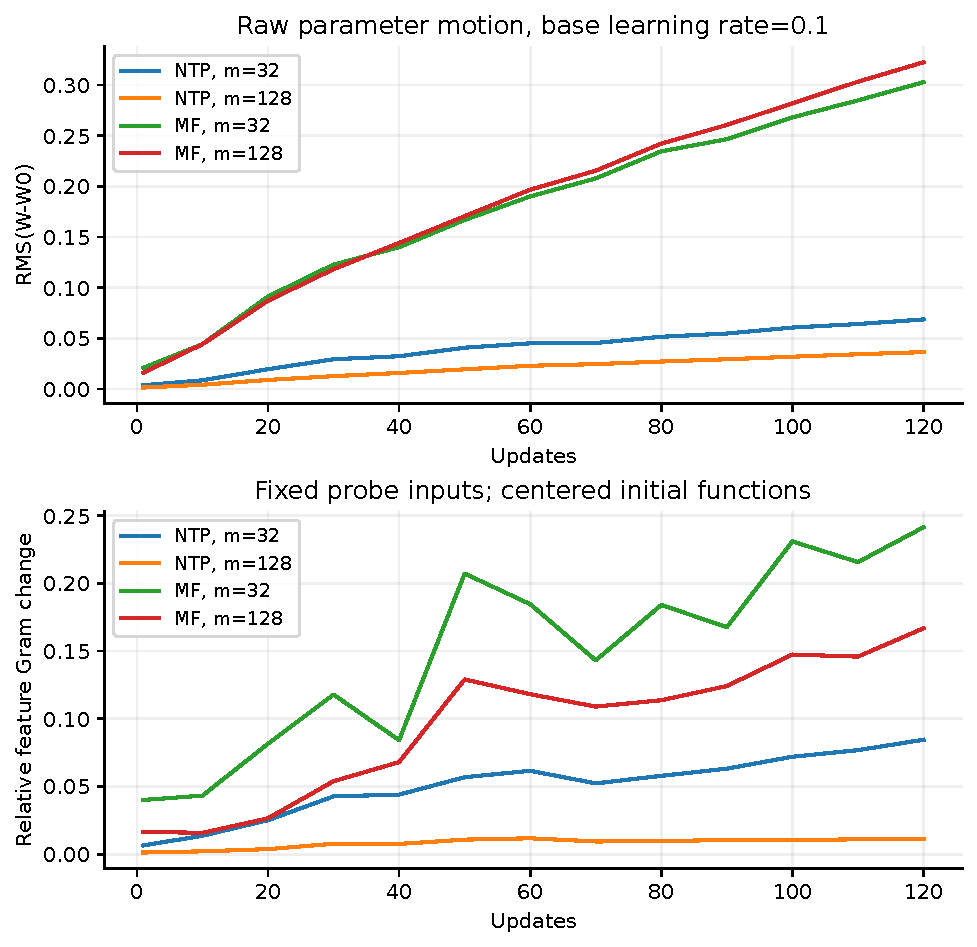
\includegraphics[width=0.85\textwidth]{figures/width_dynamics.pdf}
\caption{配套脚本的一次有限宽度运行：固定基础学习率、训练步数、batch 与探针输入，比较原始隐藏参数的移动和特征 Gram 漂移。两种参数化都减去冻结的初始函数；mean-field 使用原始参数步长 $m\eta$。这是一份单种子实验记录，图中的趋势需要通过多种子与更宽扫描检验，不能单独证明渐近尺度或性能优势。}
\label{l5:fig-width-dynamics}
\end{figure}

\section{隐式偏好、泛化与稳定性的收束}
\label{l5:closing}

\subsection{三件需要分别证明的事}

到这里，我们已经看到了三种不同层次的论断。
\begin{enumerate}
 \item \textbf{优化可达性：}给定参数化与算法，训练损失能否降低，速度与稳定范围如何？
 \item \textbf{隐式偏好：}若存在多个低损失或插值解，算法、初始化和步长倾向选择哪一类？
 \item \textbf{统计泛化：}这种被选择的解，在新的输入上是否与真实规律一致？
\end{enumerate}
最小范数结论回答第二个问题，但不单独回答第三个。因子分解的暂态谱偏好，首先描述训练路径，也不自动成为最终解的核范数定理。较大的特征漂移说明表示改变，不意味着泛化必然提升。一个完整的“适配数据”结论，应把数据或目标的结构假设加入推理链条。

\subsection{选读：局部平坦方向并不证明全局拓扑}

对平均平方损失，精确 Hessian 分解为
\begin{equation}
 \nabla_\theta^2L
 =\frac1nJ^\top J+
 \frac1n\sum_{i=1}^n r_i\nabla_\theta^2f_\theta(x_i).
 \label{l5:hessian-decomposition}
\end{equation}
在\emph{精确插值点}，残差项为零，因此 Hessian 半正定且秩至多为
$n$。若此处 $J$ 满行秩，隐函数定理进一步给出局部零损失集合是
$p-n$ 维流形，其切空间为 $\ker J$。如果只是接近插值，残差项小还需要二阶导有界，不能把近零特征值写成严格的零特征值。

这些都是局部陈述。参数个数大于样本数不单独保证整个零损失集合是一个连通流形，置换对称也不单独决定鞍点数量。关于更宽网络中某些对称极小值如何连接，已有在明确网络结构与嵌入假设下的研究\citep{Simsek2021}；本课程不把这些条件定理扩展成所有网络的拓扑定律。习题中的两神经元反例足以说明，两个等价极小值的中点甚至未必是驻点。

\subsection{Edge of Stability：对有限步长的观察}

对固定正定二次函数，普通 GD 的稳定条件为
\[
 0<\eta<\frac2{\lambda_{\max}(H)}.
\]
在一些神经网络全批量 GD 实验中，最大的 Hessian 特征值会在训练中变化，并在 $2/\eta$ 附近波动；损失在短期内可以非单调，而较长时间尺度继续降低。这类现象被称为 Edge of Stability，简称 EoS\citep{Cohen2021}。

这不违反固定 Hessian 二次目标的定理：非线性轨迹上的曲率在变，单个位置的二次近似也没有描述全部高阶动态。它提醒我们，有限步长训练可能超出单调下降和固定核近似的适用范围。

此外，$2/\eta$ 不是所有优化器共享的阈值。固定正定预条件 $P$ 下，二次模型的相关曲率是
$P^{1/2}HP^{1/2}$；带动量算法要分析含动量状态的迭代矩阵；Adam 和 Muon 还需要处理其自适应或谱变换状态。本课程的主宽度实验不以 EoS 是否出现作为成功标准，也不把原始 Hessian 变化单独当成特征学习的证据。

\subsection{选读：sharpness 与 SAM 的边界}

SAM 研究局部扰动下的目标
\begin{equation}
 \min_\theta\max_{\norm\delta_2\leq\rho}L(\theta+\delta)
 \label{l5:sam}
\end{equation}
及其可计算近似\citep{Foret2021}。在非驻点处，小半径展开首先包含
$\rho\norm{\nabla L(\theta)}_2$；在光滑驻点附近，二阶项才更直接地由 Hessian 的最大正曲率控制。因此 SAM 不能在所有位置都等同于给
$\lambda_{\max}(H)$ 加惩罚。

原始参数坐标中的 sharpness 还会随重参数化改变。某些保持网络函数不变的参数缩放，可以显著改变 Hessian 尺度，故不能无条件地用“更平坦”推出“泛化更好”\citep{Dinh2017}。这些边界并不削弱稳定性诊断的用途；它们说明解释诊断量时，必须同时说明坐标、优化器和比较协议。

\section{习题}
\label{l5:exercises}

\begin{exercise}[有效核与目标方向]
令 $F(\theta)=(\theta_1+\theta_2,\theta_1-\theta_2)^\top$，
$P=\diag(1,4)$，损失为 $\norm{F-y}_2^2/4$。
\begin{enumerate}
 \item 计算 $J$、$\mathcal K=JPJ^\top$ 与 $\Theta=\mathcal K/2$ 的特征值和特征向量。
 \item 给出普通预条件更新 $\theta^+=\theta-\eta P\nabla L$ 的稳定步长区间。
 \item 从零初始化，比较 $y=(1,1)^\top$ 与 $y=(1,-1)^\top$。取 $\eta=1/4$，分别计算一步后的残差。
 \item 找到线性坐标变换 $\theta=Su$，使对 $u$ 的欧氏 GD 与上述更新等价。
\end{enumerate}
\end{exercise}

\begin{exercise}[连续平衡与离散平衡]
设 $\ell(AB)=\norm{AB-Y}_F^2/2$，初值
$A=B=\diag(2,1)$，并取
\[
 Y=\begin{pmatrix}4&-1\\0&1\end{pmatrix}.
\]
\begin{enumerate}
 \item 计算初始梯度矩阵 $G=AB-Y$，验证初始化平衡。
 \item 用一次同时梯度更新计算 $A^+$ 与 $B^+$。
 \item 计算 $B^+(B^+)^\top-(A^+)^\top A^+$，判断离散 GD 是否精确保留平衡。
 \item 说明这一计算为何不反驳梯度流的平衡不变量。
\end{enumerate}
\end{exercise}

\begin{exercise}[宽度指数与输出坐标]
设两层模型的前向倍率为 $\kappa_m=m^{-s}$，原始 SGD 学习率为
$\eta m^t$。假设输入维度固定，初始化神经元的相关矩有界且非退化；对所讨论的有限训练区间，残差加权的单神经元梯度项保持典型 $O(1)$ 量级。
\begin{enumerate}
 \item 求有效核的典型量级及单神经元更新的典型量级。
 \item 若有效核要求保持非退化的 $\Theta(1)$ 量级，$s,t$ 应满足什么关系？若还要求单神经元更新不随宽度消失或发散，得到哪一组指数？
 \item 对 mean-field 模型令 $b=a/m$，重新推导实际输出权重的 SGD 步长。
 \item 在独立零均值输出初始化下，求原始初始输出方差关于 $m$ 的阶，并解释为什么实验需要控制初始函数。
\end{enumerate}
\end{exercise}

\begin{exercise}[对称极小值的中点反例]
考虑单样本 $x=1,y=5$，网络
\[
 f=v_1\operatorname{ReLU}(w_1x)+v_2\operatorname{ReLU}(w_2x),
 \qquad L=\frac12(f-y)^2.
\]
\begin{enumerate}
 \item 验证 $\theta=(w_1,v_1,w_2,v_2)=(1,1,2,2)$ 及其神经元交换
$\theta'=(2,2,1,1)$ 都是全局极小值。
 \item 计算中点处的预测、损失和完整梯度。
 \item 解释为什么交换对称性只强制某些反对称方向上的一阶导为零，不能推出中点是驻点。
 \item 说明该反例能够否定什么论断，以及它没有否定什么。
\end{enumerate}
\end{exercise}

\begin{exercise}[Hessian 变化是否说明特征学习]
考虑固定线性特征的单样本 logistic 模型：$F(w)=w$，正类标签下的损失
$L(w)=\log(1+e^{-w})$。
\begin{enumerate}
 \item 求预测 Jacobian $J$ 和损失 Hessian $L''(w)$。
 \item 计算 $w=0$ 与 $w\to+\infty$ 时的 Hessian，判断是否发生隐藏特征学习。
 \item 解释为什么不能仅凭训练中 Hessian 谱改变，就断言 NTK 固定核观点被反驳。
 \item 对平方损失写出式 \eqref{l5:hessian-decomposition}，说明把“近似插值”换成“精确插值”后，哪个结论从近似变成精确。
\end{enumerate}
\end{exercise}

\begin{exercise}[一份可复核的宽度迁移报告]
按第 \ref{l5:lab} 节的协议完成 NTP 与 mean-field SGD 比较。至少使用三个宽度、三个随机种子与一组共同基础学习率；训练步数和 batch 保持固定，默认中心化输出。
\begin{enumerate}
 \item 提交实际参数坐标与学习率表、原始初始输出 RMS、验证损失扫描、$D_W$ 和 $D_C$。
 \item 在查看结果之前定义“可迁移”的容忍阈值，并判断小宽度选出的学习率在较大宽度上是否满足该定义。
 \item 若 mean-field 越宽越慢，列出两个实现原因和一个模型或实验条件方面的原因，并说明如何分别核查。
 \item 若 NTP 在有限宽度下有明显特征漂移，写出一个有条件且不越界的结论。
 \item 可选做未配对 mean-field $+\eta$ 或冻结核参照，但必须说明它们各自检验的假设。
\end{enumerate}
\end{exercise}

\section{习题解答与核验要点}
\label{l5:solutions}

\subsection*{习题1：有效核与目标方向}

Jacobian 为
\[
 J=\begin{pmatrix}1&1\\1&-1\end{pmatrix},
 \qquad
 \mathcal K=\begin{pmatrix}5&-3\\-3&5\end{pmatrix},
 \qquad
 \Theta=\frac12\begin{pmatrix}5&-3\\-3&5\end{pmatrix}.
\]
沿 $q_+=(1,1)^\top/\sqrt2$ 的归一化特征值为 $1$，沿
$q_-=(1,-1)^\top/\sqrt2$ 的归一化特征值为 $4$，所以对任意初始残差都收敛的步长区间为 $0<\eta<1/2$。

第一种目标的残差 $r_0=(-1,-1)^\top$ 完全位于 $q_+$ 方向，取
$\eta=1/4$ 后变成 $r_1=(-3/4,-3/4)^\top$。第二种目标的残差
$r_0=(-1,1)^\top$ 位于 $q_-$ 方向，乘子 $1-\eta\lambda$ 等于零，一步后残差为零。相同模型、相同谱，目标投影不同便产生不同的有限步数表现。

取 $S=\diag(1,2)$，则 $SS^\top=P$。对 $u$ 作
$u^+=u-\eta S^\top\nabla_\theta L$，乘以 $S$ 后恰好得到
$\theta^+=\theta-\eta P\nabla_\theta L$。这是线性坐标下的精确等价，不涉及 Taylor 近似。

\subsection*{习题2：连续平衡与离散平衡}

初始乘积为 $AB=\diag(4,1)$，所以
\[
 G=\begin{pmatrix}0&1\\0&0\end{pmatrix},
 \qquad BB^\top=A^\top A=\diag(4,1).
\]
一次同时更新给出
\[
 A^+=\begin{pmatrix}2&-\eta\\0&1\end{pmatrix},
 \qquad
 B^+=\begin{pmatrix}2&-2\eta\\0&1\end{pmatrix}.
\]
注意第二个乘积是 $(A^+)^\top A^+$，不能在这里写成
$A^+(A^+)^\top$。直接相减得到
\[
 B^+(B^+)^\top-(A^+)^\top A^+
 =\begin{pmatrix}4\eta^2&0\\0&-\eta^2\end{pmatrix}.
\]
因此对任意非零步长都不再精确平衡。差值恰为二阶量，除以步长并令
$\eta\to0$ 后，一阶变化为零，与连续梯度流的不变量一致。若想由此获得长时间误差上界，还需要控制每一步矩阵的大小，不能只看单步的 $O(\eta^2)$。

\subsection*{习题3：宽度指数与输出坐标}

从式 \eqref{l5:two-layer-kernel} 可见，核中有 $m$ 项，每项前的系数为
$m^{t-2s}$，因此有效核的典型阶为
\[
 \mathcal K_m=O\!\left(m^{t+1-2s}\right).
\]
单神经元梯度含 $m^{-s}$，乘以学习率倍率后，更新为
$O(\eta m^{t-s})$。核保持非退化的 $O(1)$ 量级要求 $t=2s-1$；进一步要求单神经元更新既不消失也不增长，需 $t=s$。联立得到
$s=t=1$，即本讲的 mean-field 配对尺度。NTP 则是 $s=1/2,t=0$，其单神经元变化为 $O(\eta m^{-1/2})$。

对于 $b=a/m$，有 $g_a=g_b/m$，于是
\[
 \Delta b=\frac{\Delta a}{m}
 =-\frac{m\eta}{m}\,g_a
 =-\frac\eta m g_b.
\]
所以实际输出学习率为 $\eta/m$，而非 $m\eta$。

在独立零均值初始化下，原始输出方差为 $O(m^{1-2s})$，对应 RMS 为
$O(m^{1/2-s})$。NTP 的 RMS 为 $O(1)$，mean-field 为
$O(m^{-1/2})$。若不控制初始函数，比较会同时改变起点、参数化和更新尺度；默认中心化将起点固定为零，但仍应记录原始 RMS 检查初始化实现。

这些阶关系依赖题设中的典型非退化贡献。若数据、标签或参数处于特殊对称状态，某些梯度可以精确为零；量级分析不允许把这样的零量强行认作一般 $O(1)$ 信号。

\subsection*{习题4：对称极小值的中点反例}

两个端点的预测分别都是 $1\cdot1+2\cdot2=5$，损失为零，故均为全局极小值。中点四个参数都等于 $1.5$；由于隐藏输入为正，ReLU 在此可微。其预测为 $4.5$，残差为 $-0.5$，损失为 $0.125$。

对每个神经元，$\partial f/\partial w_r=v_r=1.5$、
$\partial f/\partial v_r=w_r=1.5$，所以
\[
 \nabla_\theta L=(-0.75,-0.75,-0.75,-0.75)^\top.
\]
中点不是驻点，更谈不上由 Hessian 分类的鞍点。

将两神经元写成平均部分与差分部分后，交换对称性使损失关于差分的联合符号翻转不变，故差分为零时的反对称一阶导为零。但平均部分的导数不必为零，端点的驻定条件也不会自动传给它们的平均。该反例否定的是“任意置换等价极小值的中点必为驻点或鞍点”的普遍说法。它没有否定置换等价性，也没有否定在额外条件下构造低损失连接路径或某些对称临界点的研究结果。

\subsection*{习题5：Hessian 变化与固定特征}

令 $s(w)=1/(1+e^{-w})$，则
\[
 J=1,\qquad L'(w)=s(w)-1,
 \qquad L''(w)=s(w)(1-s(w)).
\]
在 $w=0$ 时 Hessian 为 $1/4$，在 $w\to+\infty$ 时趋于零。模型的预测 Jacobian 一直为常数，没有任何隐藏特征可学习；变化来自损失对预测的曲率。因此，非平方损失下，即使 $JJ^\top$ 固定，参数损失 Hessian 仍可能变化。不能仅测 Hessian 就断言特征学习发生，也不能据此否定固定核的条件性理论。

平方损失的分解为
\[
 H=\frac1nJ^\top J+\frac1n\sum_i r_i\nabla^2f_i.
\]
在精确插值点，第二项严格为零，故 $H=J^\top J/n$、$H\succeq0$、
$\rank H\leq n$ 都是精确结论。在近似插值点，若二阶导有界，第二项才可被上界为一个小扰动；小扰动可以使原本的零特征值变成正或负的小数，不能继续声称 Hessian 严格低秩。

\subsection*{习题6：实验报告的判断方法}

这道题没有事先指定的一组数值曲线。可复核的答案首先应当确认三个配置层次：前向系数、实际存储变量和实际学习率相互一致；数据与训练预算固定；初始函数经过同样的中心化。漏掉任何一层，后续曲线都不能直接解释为宽度效应。

一个可接受的迁移定义可以是：在最小宽度上用验证集选出的基础学习率，在其他宽度均不发散，并且各自最终验证损失不超过该宽度扫描最优值加预先给定的容忍量。容忍量应在查看测试结果之前确定，且最好同时报告整个近最优区间，避免把极小的随机差异解释为迁移失败。

若 mean-field 越宽越慢，可先检查原始 $a,W$ 的步长是否错误地保持为
$\eta$，以及 forward 或 loss 是否重复除以宽度。第一项可通过打印参数组与一次手算更新核查，第二项可通过同一 batch 的手算损失和梯度尺度核查。若实现无误，还应检查基础步长是否过小、固定预算是否只覆盖了不同宽度的暂态，以及数据或初始化是否导致退化梯度；此时可以增加一个受控步长或训练时间对照，但不能在主扫描中悄悄改变预算。

若有限宽度 NTP 有明显特征漂移，合格结论应指出具体宽度、学习率和训练步数，并说“这一配置尚未接近固定特征近似”。还可以检查随宽度增大漂移是否减小，或与冻结核参照比较。不能直接推导“NTK 错误”，也不能反过来因理论预期而删去该实验。

未配对 mean-field 负对照主要检验前向与步长是否配平；冻结核参照主要检验固定 Jacobian 是否足以解释当前预测动态。前者不是统计泛化对照，后者也不能在随机 batch 协议不同的情况下独自定位特征学习来源。

\section{本讲概念检查}
\label{l5:checklist}

回到课程开头的问题：“从优化器角度，如何设计网络去适配数据？”本讲提供的回答步骤是：先写出实际参数化与更新，再得到数据上的有效几何；识别目标落在哪些方向，研究这些方向在初始化及训练过程中如何变化；最后通过固定预算的宽度扫描检验缩放与迁移。任何一步都需要可核验的假设或观测。

离开本讲前，应能独立解释以下区别：$JPJ^\top$ 与参数 Hessian、内部 Gram 平衡与左右输出 Gram、原始 $a$ 与实际输出 $b$、固定时间宽度极限与长时间训练、表示变化与泛化改善。能够说明这些区别，比记住一个没有坐标约定的“最佳学习率倍率”更有用。
